\chapter{RZ- und IT-Management}

\section{Sie kennen die wichtigsten IT-Betriebsprozesse und	verstehen die Bedeutung des IT-Betriebs für ein	Unternehmen.}

Man muss zwischen IT-Unternehmen und IT-Abteilungen in Unternehmen unterscheiden.

\subsection{Was macht die IT-Abteilung in einer Unternehmung / Was ist ihr Zweck? (MEP)}
\begin{itemize}
	\item Mittels IT-Services werden die Geschäftsprozesse (Kernprozesse) unterstützt. Die Folge daraus ist, dass man den Umsatz steigern möchte oder Kosten senken.
	\item Nehmen Anforderungen auf und \textbf{entwickeln} Software. Klassische Softwareentwicklung. Dazu gehört auch Applikations-Einkauf.
	\item 'Entwickelte' Software müssen \textbf{betrieben} werden
\end{itemize}
Randbemerkung: Die Entwicklung hat der Druck zu Veränderungen und der Betrieb möchte möglichst keine Veränderungen (Konstanz).

\begin{figure}[h]
	\centering
	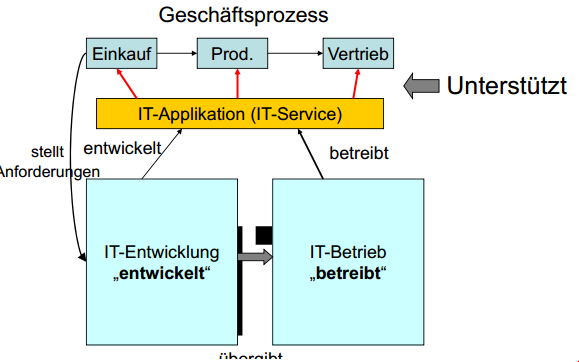
\includegraphics[width=0.7\linewidth]{fig/zweck-der-it}
	\caption{Zweck der IT}
\end{figure}

\subsection{IT-Betrieb}
Das Ziel des IT Betriebs ist ganz klar, dass die Services verfügbar sein müssen. Dafür benötigt es eine hochstehende Applikationsentwicklung, Qualitätssicherung und Kontrolle, Infrastruktur, Aufbau-Organisation sowie IT-Betriebsprozesse.

\subsubsection{Operationsmodi im IT-Betrieb}
\begin{itemize}
	\item Normal Operation (Daily Business)
	\item Change Operation (Ständige Neu-Entwicklung, Hardware ausbauen, ist die grösste Fehlerquelle)
	\item Problem Operation (Es gibt immer Probleme)
\end{itemize}

\subsubsection{IT-Betriebsprozesse}
\begin{description}
	\item[Management-Prozesse] \hfill
	\begin{description}
		\item[Service Level Management] \hfill \\
			Definiert, überwacht und optimiert die IT-Service Vereinbarungen mit dem Business.
		\item[IT-Service Continuity Management] \hfill \\
			Stellt die Wiederherstellung von Anwendungen, Plattformen und Daten durch Vorsorgemassnahmen sicher und überprüft und testet diese periodisch.
		\item[Architektur und Standards] \hfill \\
			Legt die Architektur und Standards für den IT-Betrieb fest. Dies umfasst Hardware, Software (z.B. welche Datenbanken) und IT-Betriebsapplikationen.
		\item[Plattform-Management] \hfill \\
			Erstellt und wartet Runtime-Plattformen für die IT. Eine Plattform umfasst Hard- und Software.
	\end{description}
	\item[Kernprozesse] \hfill
	\begin{description}
		\item[Monitoring] \hfill \\
			Effektive und potentielle Störungen erkennen und automatische Massnahmen zur Behebung auslösen.
		\item[Incident Management] \hfill \\
			Stellt bei Beeinträchtigung eines Services diesen so schnell als möglich wieder her.
		\item[Problem Management] \hfill \\
			Hält Fehlerhäufigkeit möglichst gering und verhindert das wiederholte Auftreten von Störungen.
		\item[Change Management] \hfill \\
			Managed alle Änderungen an Software / Hardware und Netzen mittels standardisierten Verfahren.		
		\item[SW/HW Deployment / Release Management] \hfill \\
			Plant und führt den Rollout von getesteter Hard- und Software durch.		
		\item[Service Desk] \hfill \\
			Der Service Desk (Help Desk) ist die zentrale Anlaufstelle für den Kunden.		
	\end{description}
	\item[Unterstützungsprozesse]
	\begin{description}
		\item[Configuration Management] \hfill \\
			Führt den Status aller IT Komponenten und deren Beziehungen und stellt diese Informationen allen anderen ICT Prozessen zur Verfügung.
		\item[Capacity Management] \hfill \\
			Plant und verwaltet die für den IT Betrieb nötigen technischen Ressourcen (Storage, RAM, CPU, ...).
		\item[Availability Management] \hfill \\
			Stellt die vereinbarte Verfügbarkeit und die Performance der IT Services sicher.
		\item[Financial Management of IT Services] \hfill \\
			Regelt und wickelt die Bezahlung von IT Services ab. IT als Dienstleister innerhalb eines Unternehmens.
	\end{description}
\end{description}

\section{Sie kennen den Incident-Management Prozess und können Key Performance Indikatoren und Critical Success Factors erläutern.}
\label{sec:incident-management}

\subsection{Ziel}
Das Ziel des Incident Management Prozesses ist die schnelle Behebung von Störungen. Dabei werden oft temporäre Lösungen (Workarounds) eingesetzt, um die Services möglichst schnell wieder verfügbar zu machen - was zufriedene Nutzer bedeutet.

\subsection{Ablauf}
Abbildung \ref{fig:ablauf-incident-management} zeigt die Aktivitäten eines einfachen Incident Management Prozesses. Der Prozess kann in verschiedenen Unternehmen sehr unterschiedlich sein und an die Anforderungen des Unternehmens angepasst sein.

\begin{figure}[h!]
	\centering
	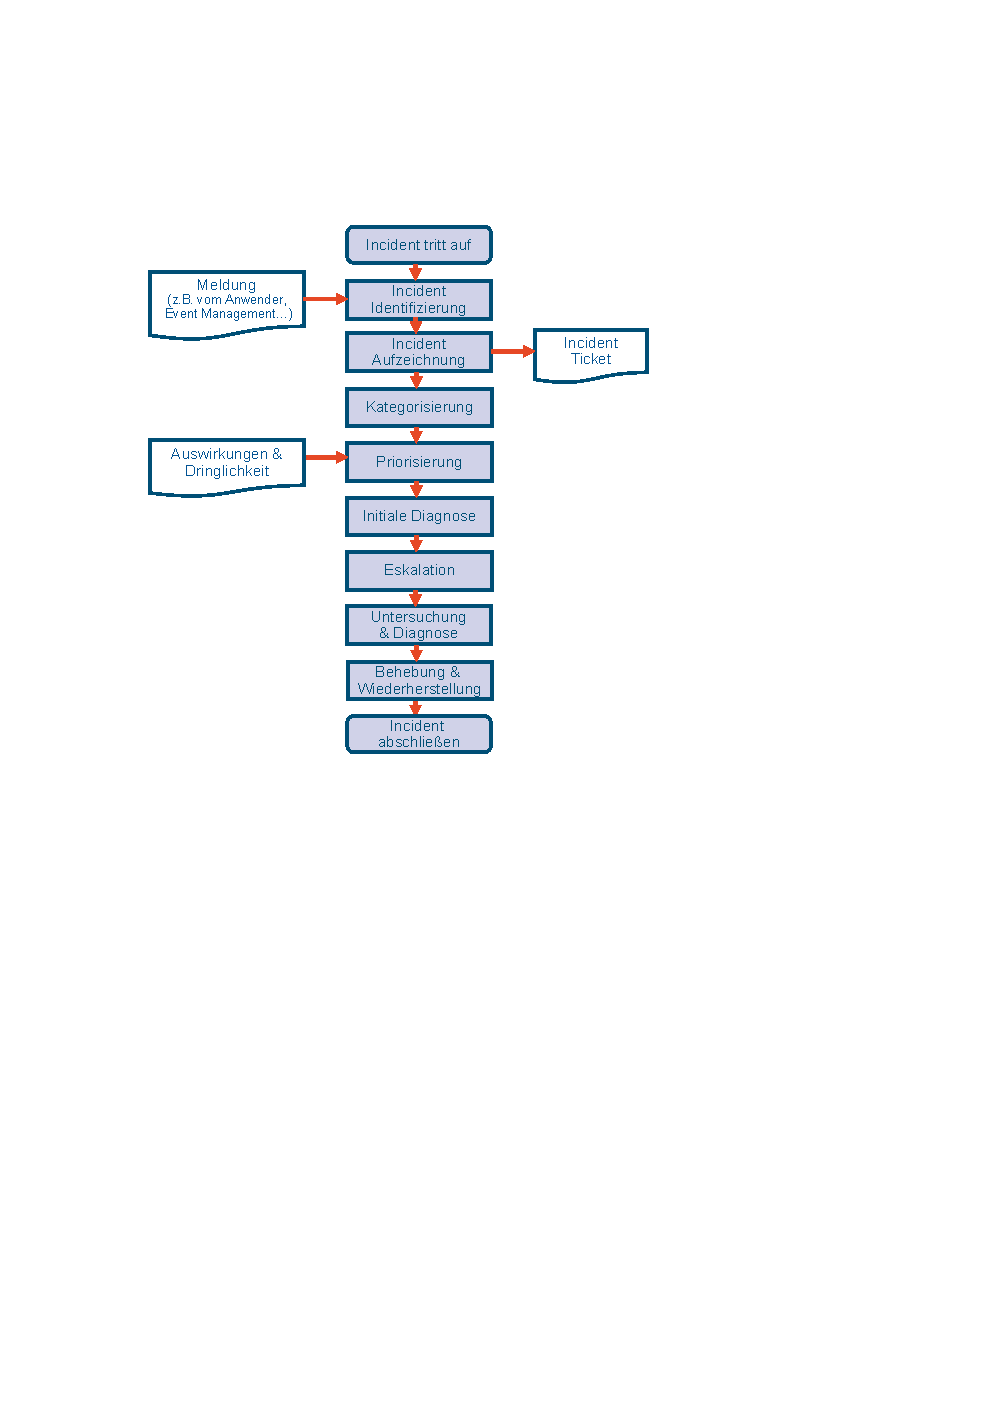
\includegraphics[width=0.7\linewidth]{fig/ablauf-incident-management}
	\caption{Aktivitäten eines Incident Management Prozesses}
	\label{fig:ablauf-incident-management}
\end{figure}

\subsection{Rollen}
\begin{description}
	\item[Incident Manager:] Der Incident Manager ist verantwortlich für einen funktionierenden Prozess und stellt sicher, dass die Aktivitäten innerhalb dieses Prozesses effektiv und effizient erfolgen.
	\item[1st Line Support:] Der 1st Line Support nimmt Anrufe entgegen und versucht Incidents mithilfe einer Knowledge Base zu lösen. Ungefähr 80\% aller Incidents können hier gelöst werden. Dauert die Bearbeitung aber länger als ca. eine halbe Stunde wird der Incident an den 2nd Line Support weitergegeben.
	\item[2nd Line Support:] Weitergeleitete Incidents werden von Engineers des IT-Betriebs behandelt. Der 2nd Line Support ist meisten nicht die Hauptaufgabe dieser Teams. Er arbeitet ohne Zeitlimit am Problem.
	\item[3rd Line Support:] Beim 3rd Line Support werden die (Inhouse) Entwickler geweckt. Bei externen Dienstleistern (z.B. Oracle) wird zusammen mit den Inhouse Entwicklern nach Lösungen genutzt.
\end{description}

\subsection{Key Performance Indicator}
\begin{itemize}
	\item Wie viele Störungen treten auf? 
	\item Wie lange dauert es durchschnittlich bis die Störung behoben ist? 
	\item Wie viel Prozent der Störungen kann der First-Level Support direkt beheben?
\end{itemize}

\subsection{CSF - Critical Success Factors}
Für den Erfolg des Incident Management Prozesses sind folgende Punkte essentiell:
\begin{itemize}
	\item Aktuelle CMDB, damit die Auswirkung einer Störung eingeschätzt werden kann, um die Prirosierung korrekt zu machen.
	\item Behobene Fehler an zentralem Ort dokumentieren, damit bei wiederkehrenden Problemen darauf zurückgegriffen werden kann.
	\item System zur Erfassung, Verfolgung und Überwachen von Störungen vom Auftreten bis zur Lösung.
	\item Enge Beziehung zum Service Level Management, um festzustellen, wie dringend der Service wiederhergestellt werden muss.
\end{itemize}